% Copyright (C) 2011 The ESPResSo project
%   Max-Planck-Institute for Polymer Research, Theory Group
%  
% This file is part of ESPResSo.
%   
% ESPResSo is free software: you can redistribute it and/or modify it
% under the terms of the GNU General Public License as published by the
% Free Software Foundation, either version 3 of the License, or (at your
% option) any later version.
%  
% ESPResSo is distributed in the hope that it will be useful, but
% WITHOUT ANY WARRANTY; without even the implied warranty of
% MERCHANTABILITY or FITNESS FOR A PARTICULAR PURPOSE.  See the GNU
% General Public License for more details.
%  
% You should have received a copy of the GNU General Public License
% along with this program.  If not, see <http://www.gnu.org/licenses/>.
%
\documentclass[
a4paper,                        % paper size
11pt,                           % font size
twoside,                        % two sided
footsepline,                    % add a line to separate the footer
headsepline,                    % add a line to separate the header
headexclude,                    % header does not belong to the text
footexclude,                    % footer does not belong to the text
pagesize,                       % set the pagesize in a DVI document
bibtotocnumbered,               % add the bibliography to the TOC
idxtotoc                        % add the index to the TOC
%openright,                      % start a new chapter on the right page
%,DIV12
%,draft
]{scrartcl}

\usepackage[draft]{varioref}    % defines \vref
\usepackage{hyperref}           % automatically creates links when
                                % using pdflatex, defines \url
\usepackage{ifpdf}              % defines \ifpdf
\usepackage{graphicx}           % handles graphics
\usepackage{makeidx}            % creates the index
\usepackage{color}              % use colors

\usepackage{amsmath}

\usepackage{calc}               % compute length
\usepackage{ifthen}             % provide ifthen
\usepackage{xspace}
\usepackage{units}
\usepackage[numbers]{natbib}

% For building the distribution docs, disable todo boxes.
%\usepackage[disable]{todonotes}
\usepackage{todonotes}

%%%%%%%%%%%%%%%%%%%%%%%%%%%%%%%%%%%%%%%%%%%%%%%%%%
%%%%%%%%%%%%%%%%%%%%%%%%%%%%%%%%%%%%%%%%%%%%%%%%%%
%%%%%%%%% New Commands and Environments %%%%%%%%%%
%%%%%%%%%%%%%%%%%%%%%%%%%%%%%%%%%%%%%%%%%%%%%%%%%%
%%%%%%%%%%%%%%%%%%%%%%%%%%%%%%%%%%%%%%%%%%%%%%%%%%
\newcommand{\es}{\mbox{\textsf{ESPResSo}}\xspace}
\newcommand{\ie}{\textit{i.e.}\xspace}
\newcommand{\eg}{\textit{e.g.}\xspace}
\newcommand{\etal}{\textit{et al.}\xspace}


%%%%%%%%%%%%%%%%%%%%%%%%%%%%%%%%%%%%%%%%%%%%%%%%%%
%%%%%%%%%%%%%%%%%%%%%%%%%%%%%%%%%%%%%%%%%%%%%%%%%%
%%%%%%%%%%%%%%%% Other Settings %%%%%%%%%%%%%%%%%%
%%%%%%%%%%%%%%%%%%%%%%%%%%%%%%%%%%%%%%%%%%%%%%%%%%
%%%%%%%%%%%%%%%%%%%%%%%%%%%%%%%%%%%%%%%%%%%%%%%%%%
\makeindex

%%%%%%%%%%%%%%%%%%%%%%%%%%%%%%%%%%%%%%%%%%%%%%%%%%
%%%%%%%%%%%%%%%%%%%%%%%%%%%%%%%%%%%%%%%%%%%%%%%%%%
%%%%%%%%%%%%%%%%% Main Document %%%%%%%%%%%%%%%%%%
%%%%%%%%%%%%%%%%%%%%%%%%%%%%%%%%%%%%%%%%%%%%%%%%%%
%%%%%%%%%%%%%%%%%%%%%%%%%%%%%%%%%%%%%%%%%%%%%%%%%%
\begin{document}
\titlehead{
  \begin{center}
    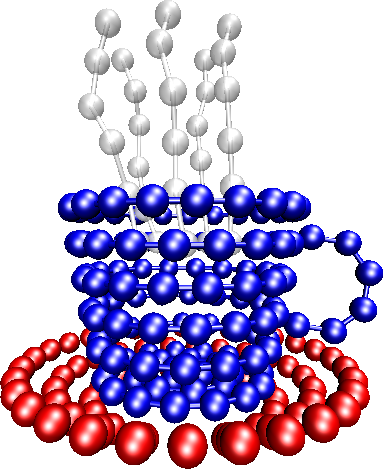
\includegraphics[width=5cm]{logo/transparentbg.png}
  \end{center}
}
%\subject{}
\title{\es Developer's Guide}
%\author{}
%\date{\today}
\maketitle

\tableofcontents

\section{Development environment}
\label{sec:env}

\begin{itemize}
\item Autotools build system
\item \es homepage \url{http://espressomd.org}
\item Code hosting at GNU Savannah 
  \url{https://savannah.nongnu.org/projects/espressomd/}
\item Jenkins build server \url{http://espressomd.org/jenkins}
\end{itemize}

\section{Getting into contact}

The first thing that you should do when you want to start to
participate is to get into contact with the \es developers. To do
that, subscribe to the developers' mailing list at
\url{http://lists.nongnu.org/mailman/listinfo/espressomd-devel} and
write a short email to the list address
\texttt{espressomd-devel@nongnu.org} where you state your experience
with simulations and programming and the things that you would like to
do in \es. We do not bite, and we are happy about anybody who wants to
participate!

\section{Required development tools}
\label{sec:requirements}

If you want to participate in the development of \es, you will require
the following tools depending on what tasks you want to perform:

\begin{itemize}
\item To be able to access the development version of \es, you will
  need the distributed versioning control system
  Git\footnote{\url{http://git-scm.com/}}.  Section \vref{sec:git}
  contains documentation on how we employ git.
\item To build \es from the development sources, you will need not too
  old versions of the ``GNU autotools'' (\ie
  automake\footnote{\url{http://www.gnu.org/software/automake/}} and
  autoconf\footnote{\url{http://www.gnu.org/software/autoconf/autoconf.html}})
  installed on your system. Section \vref{sec:build_devel} contains
  information on how to build the development code, section
  \vref{sec:build_system} contains details on how the build system
  works.
\item To be able to compile the User's Guide or the Developer's Guide,
  you will need a \LaTeX-installation (all recent ones will do). For
  details, refer to chapter \vref{sec:docs}.
\item To compile the Doxygen code documentation, you will need to have
  the tool \textsc{Doxygen}\footnote{\url{http://www.doxygen.org/}}.
\end{itemize}

All of these tools should be easy to install on most Unix operating
systems.

\section{Using git}
\label{sec:git}

\section{Building the development code}
\label{sec:build_devel}

\begin{itemize}
\item Use \texttt{bootstrap.sh} before building the code.
\item Use configure with \texttt{--enable-maintainer-mode}.
\item Possible targets of \texttt{make}
  \begin{itemize}
  \item \texttt{check}
  \item \texttt{dist}
  \item \texttt{doc}
  \item \texttt{ug}
  \item \texttt{dg}
  \item \texttt{doxygen}
  \item \texttt{tutorials}
  \item \texttt{distcheck}
  \item \texttt{clean}, \texttt{distclean}
  \end{itemize}
\end{itemize}

\section{The Build System}
\label{sec:build_system}

The build system of ESPResSo makes use of the GNU autotools suite
consisting of
automake\footnote{\url{http://www.gnu.org/software/automake/}} and
autoconf\footnote{\url{http://www.gnu.org/software/autoconf/autoconf.html}}.
If you want to use the development source code of ESPResSo, you first
need to install both of these tools.

The central source files of the build system are the following:
\begin{itemize}
\item \texttt{configure.ac}
\item \texttt{config/*.m4}
\item \texttt{Makefile.am}
\item the different \texttt{Makefile.am} in the subdirectories
\end{itemize}

To change the behaviour of the build system, you have to modify any
these files.

\subsection{Running \texttt{bootstrap.sh}}

The script \texttt{bootstrap.sh} in the top level source directory can
be used to run \texttt{automake}, \texttt{autoconf} and the associated
tools to generate the \texttt{configure} script and the
\texttt{Makefile.in} used during compilation.  Once
\texttt{bootstrap.sh}, the \es development code can be build and used
like the release code.

\subsection{Creating a distribution package}

As described in the User's Guide, to create a \texttt{.tar.gz}
distribution file that contains all required files, you can simply run
\texttt{make dist}. This will bundle all files and put them into an
archive with the name
\texttt{espresso-\textit{version}\texttt{.tar.gz}}.

Even better, you can also run \texttt{make distcheck}. This will not
only create the distribution file, but it will also thoroughly check
the created distribution, \ie it will try to 
\begin{itemize}
\item unpack the distro into a new directory
\item configure and build it (\texttt{configure})
\item run the testsuite (\texttt{make check})
\item install it into a new directory (\texttt{make install})
\item uninstall it (\texttt{make uninstall})
\end{itemize}
Whenever something goes wrong in these checks, it will give an error
message that describes the problem. When everything goes fine, you can
be relatively sure that you have a useful \es distribution
package.

In some cases, it might be necessary to pass some options to the run
of \texttt{configure} done by \texttt{make distcheck}>. To these ends,
the environment variable \texttt{DISTCHECK\_CONFIGURE\_FLAGS} can be
set to the required options.

\paragraph{Example}
\begin{verbatim}
DISTCHECK_CONFIGURE_FLAGS="--without-mpi CPPFLAGS=\"-I /usr/include/tcl8.4\"" \
  make distcheck
\end{verbatim}

\subsection{Adding new files}

To add new files to \es (like C source files or header files)
you need to do the following:
\begin{itemize}
\item Add the files to the \texttt{Makefile.am} in the same directory
\item Run \texttt{bootstrap.sh} in the source directory
\item Check the distribution by using \verb!make distcheck!
\item Add the files to the Git repository
\end{itemize}

\section{The Testsuite}
\label{sec:testsuite}

\begin{itemize}
\item How to write tests?
\item How they are called (\texttt{runtest.sh})
\end{itemize}

\section{Doxygen Code Documentation}
\label{sec:doxygen}

The documentation of each function should contain a short description,
if necessary a more detailed description and a description for the
return value and parameters.

Look at the documentation of existing files and functions to get a
feeling how it should be!

Doxygen is able to understand simple \LaTeX\ and HTML commands as well
as some special command in order to give the documentation a nice
structure and to make it more readable. In the following list you find
a short description of the most common commands we need:

\begin{itemize}
\item \verb!\anchor! \textit{name} \textit{description}\\
  Create an anchor to which you can refer using the \verb!\ref!
  command.
\item \verb!\ref! \textit{name} \texttt{["}\textit{text}\texttt{"]}\\
  Insert a link to another object in the documentation (\eg an
  anchor).
\item \verb!<a href="http://www.your_url.html">title</a>!\\
  Link to an external HTML source.
\item \verb!\file! \textit{name} \textit{description}\\
  Special anchor for a file.
\item \verb!\image html! \textit{image}\\
  Include a picture. The picture file should reside in the subdir
  \verb!doc/doxygen/figs!. Do not use the HTML \verb!<img>!-tag to
  include pictures, as doxygen will not copy the pictures into the
  documentation.
\item \verb!<ul> <li>List entry 1</li> <li>List entry 2</li></ul>!\\
  Creates a list in the documentation.
\item \verb!\param! \textit{name} \textit{description}\\
  Document the parameter of a function.
\item \verb!\return! \textit{decription}\\
  Document the return value of a function.
\end{itemize}

\section{User's Guide}

The User's Guide is written in \LaTeX. The source files reside in the
subdirectory \texttt{doc/ug/} of the \es sources. The master file is
\texttt{ug.tex}, each chapter is contained in its own source file.

\subsection{General issues}

\begin{itemize}
\item Other than usual, in the UG's \texttt{.tex}-files, the
  underscore character ``\_'' is a normal character in most cases, \ie
  it can be used unquoted. Unfortunately, however, this makes it
  impossible to use ``\_'' in \LaTeX-labels (don't ask me why!).
\item Headings should start with a capital letter and continue with
  lower-case letters (``First steps'' and \emph{not} ``First Steps'').
\item Use the ``-ing'' form in headings, \ie ``Setting up particles''
  instead of ``Particle setup'' or the like.
\item To see which parts of the User's guide need to be fixed or which
  documentation is missing, there is a \verb!\todo!-command where one
  can put notes about what remains to be done. In the release version,
  the boxes are diabled so that they do not disturb the users. They
  can be turned on by commenting out the appropriate line in
  \texttt{ug.tex}:
\begin{verbatim}
%% For building the distribution docs, disable todo boxes.
%\usepackage[disable]{todonotes}
\usepackage{todonotes}
\end{verbatim}

\end{itemize}

\subsection{Building the User's Guide}
\begin{itemize}
\item To build the User's Guide, you need to have a \LaTeX-installation
  that includes BibTeX, PDFLaTeX and makeindex. All installations that
  I know of provide these tools.
\item There are two methods to build the User's Guide:
  \begin{itemize}
  \item Use \texttt{make ug} from the build directory to build
    it. This will automatically generate the \es quick reference
    and call latex, bibtex and makeindex as required.
  \item Use \texttt{perl latexmk} from the source directory. This will
    basically do the same, however, it will \emph{not} automatically
    update the quick reference. The advantage of this method is, that
    you can use all of \texttt{latexmk}'s nice features, such as
    \texttt{-pvc}. You can always rebuild the quick reference manually
    by calling 
    \begin{verbatim}
awk -f assemble_quickref.awk > quickref.inp
    \end{verbatim}
  \end{itemize}
\end{itemize}

\subsection{Adding new files}

To add new \LaTeX-files to the User's Guide, you need to modify
\begin{itemize}
\item \texttt{ug.tex}: add an appropriate include command near the end
  of the file
\item \texttt{Makefile.am}: add the file to the variable
  \texttt{ug\_TEXFILES}. 
\end{itemize}

\subsection{Additional environments and commands}

To maintain a consistent layout, a number of environments and
commands have been defined that should be used where applicable. 
\begin{itemize}
\item For the description of \es's Tcl-commands, read \ref{tcl_docs}.
\item The name of \es should be set via the command \verb!\es!.
\item The strings ``\ie'', ``\eg'' and ``\etal'' should be set via
  \verb!\ie!, \verb!\eg! and \verb!\etal!.
\item For short pieces of code that can be displayed inline, use
  \verb!\codebox{!\textit{text}\verb!}! or \verb|\verb!|\textit{text}\verb|!|
\item For longer code pieces or the syntax decription of non-Tcl
  commands, the environment \texttt{code} exists:
\begin{verbatim}
\begin{code}
  ...
\end{code}
\end{verbatim}
  Note that this is \emph{not} a verbatim environment, \ie it will
  evaluate \LaTeX-commands that are used inside. Therefore, the
  characters \verb!\!, \verb!{! and \verb!}! need to be quoted with
  backslashes inside the environment!  Also, the underscore character
  ``\_'' needs to be quoted like \verb!\_!. On the other hand, it is
  possible to use other layout commands (like \verb!\textit!) inside.
\item For pieces of Tcl-code that make extensive use of \verb!{! and
    \verb!}!, a verbatim environment \verb!tclcode! exists: 
\begin{verbatim}
\begin{tclcode}
 ...
\end{tclcode}
\end{verbatim}
\end{itemize}

\subsection{Documentation of Tcl commands}
\label{tcl_docs}

\subsubsection{Formal syntax definition}

All \es-commands have to be documented in the User's Guide.

The command
\verb!\newescommand[!\textit{label}\verb!]{!\textit{command}\verb!}!
should be used at the beginning of a command description to generate a
label \verb!es:!\textit{command} and create appropriate index
entries. The optional argument \textit{label} is only required, when
\textit{command} contains an underscore character ``\_''. In that
case, a label \verb!es:!\textit{label} is generated that should not
contain an underscore character.

For the \emph{formal syntax definition}, you have to use the
environments \texttt{essyntax} or \texttt{essyntax*}.  Both will
generate the headings \emph{Syntax} and
\emph{Description}. \texttt{essyntax} will furthermore copy the syntax
definition to the quick reference guide.  For an example, look at the
documentation of the \texttt{part} command in the file
\texttt{part.tex}. Inside the \texttt{essyntax} environment, you have
to use the following commands for typesetting the definition:
\begin{itemize}
\item \verb!\variant{!\textit{number}\verb!}! to typeset the label of a
  command variant
\item \verb!\var{!\textit{name}\verb!}! to typeset a variable
  argument. Note, that the argument is typeset in math mode.  This
  means, that you can use ``\_'' to denote a subscript.
\item \verb!\keyword{!\textit{text}\verb!}! or
  \verb!\lit{!\textit{text}\verb!}! to typeset keywords or literals.
\item \verb!\opt{!\textit{text}\verb!}! to typeset optional
  arguments. Note that usually, the text inside the \texttt{opt}
  command will not be wrapped. If the optional argument is pretty long
  and needs to be wrapped, use \verb!\optlong!.
\item \verb!\optlong{!\textit{text}\verb!}! to typeset long optional
  argument blocks.
\item \verb!\alt{!\textit{alt1} \verb!\asep! \textit{alt2}
    \verb!\asep! \textit{alt3} \dots \verb!}! to typeset alternatives.
\item \verb!\feature{!\textit{feature}\verb!}! to typeset when a
  \textit{feature} is referred to.
\item \verb!\require{!\textit{number}\verb!}{!\textit{text}\verb!}! to
  typeset \textit{text} to show that it requires certain features of
  \es. \textit{number} denotes the marking that is shown next to
  \textit{text}. When this command is used, you also have to use the
  \texttt{features}-environment (see below) at the end of the
  \texttt{essyntax} environment, where all of the \textit{number}s
  used are explained.
\item The environment \texttt{features} to typeset which features are
  required by the Tcl-command. Inside the environment, each feature
  should be declared via the command
  \verb!\required[!\textit{number}\verb!]{!\textit{feature}\verb!}!,
  where the optional argument \textit{number} is the number used above
  and \textit{feature} is the feature in capital letters.
\end{itemize}

The formal syntax definition should be as simple and as readable as
possible, as it will be what a user references to. Avoid very long
definitions and constructs like nested alternatives and options.  In
those cases, prefer to split the syntax definition into several
variants instead of writing it in a single, complicated definition.

\paragraph{Example}
\begin{verbatim}
\begin{essyntax}
[clip]
\variant{5} constraint pore 
  center \var{c_x} \var{c_y} \var{c_z} 
  axis \var{n_x} \var{n_y} \var{n_z} 
  radius \var{rad}
  length \var{length} 
  type \var{id} 

\require{1}{%
  \variant{6} constraint rod center \var{c_x} \var{c_y} 
  lambda \var{lambda}
} 
  
\require{1}{%
  \variant{7} constraint plate height \var{h}
  sigma \var{sigma} 
}
  
\require{2,3}{%
  \variant{8} constraint ext_magn_field \var{f_x} \var{f_y} \var{f_z} 
}

  \begin{features}
  \required{CONSTRAINTS}
  \required[1]{ELECTROSTATICS}
  \required[2]{ROTATION}
  \required[3]{DIPOLES}
  \end{features}
\end{essyntax}
\end{verbatim}

\subsubsection{Description}

In the description, you should use all of the above typesetting
commands when you refer to them in the text.  In particular, every
variable argument introduced via the \verb!\var!-command in the
definition has to be explained in detail:
\begin{itemize}
\item state explicitly the \emph{type} of the argument (integer,
  float, string, Tcl-list)
\item explain the meaning of the argument
\end{itemize}

If the command has a number of different options, \ie independent,
optional arguments, they can be described in the \emph{arguments}
environment:
\begin{verbatim}
\begin{arguments}
  \item[<arg1>] <description of arg1>
  \item[<arg2>] <description of arg2>
  ...
\end{arguments}
\end{verbatim}

The environment will generate the subheading \emph{Arguments} and
nicely format the descriptions.

\paragraph{Example}
\begin{verbatim}
\begin{arguments}
  \item[\opt{\alt{short \asep verbose}}] Specify, whether the output is
    in a human-readable, but somewhat longer format (\keyword{verbose}),
    or in a more compact form (\keyword{short}). The default is
    \keyword{verbose}.
  
  \item[\opt{\alt{folded \asep absolute}}] Specify whether the particle
    positions are written in absolute coordinates (\keyword{absolute})
    or folded into the central image of a periodic system
    (\keyword{folded}). The default is \keyword{absolute}.
  
  ...
\end{arguments}
\end{verbatim}

\end{document}
